\documentclass[12pt]{article}
\usepackage[margin=1in]{geometry}
\usepackage{amsmath}
\usepackage{amsthm}
\usepackage{float}
\usepackage{graphicx}
\usepackage{natbib}
\usepackage{enumitem}
\usepackage{booktabs}
\usepackage{hyperref}
\usepackage[utf8]{inputenc}
\usepackage{lipsum}
\usepackage[english]{babel}
\usepackage[autostyle, english = american]{csquotes}
\usepackage{underscore}
\MakeOuterQuote{"}
\title{Call Center Regression Data Analysis}

\author{Michael  Marcaccio}

\date{November 14 2022}

\begin{document}

\maketitle

\begin{abstract}
 With over 15 million people employed, a compound annual growth rate (CAGR) of 5.6 percent between 2020 and 2027, and 28,000
 in the United States alone, call centers play a pivotal role in a businesses success.In this paper, call center volume was forecasted and
 models were created to predict the number of agents needed to meet critical attributes such as waittime, calltime, and holdtime. 
 Forecasting gives businesses the ability to make informed business decision and develop data-driven strategies. In the literature it is very
 common to see call center volume being predicted using different techniques, but there is very limited studies on attempting to correlate
 the number of agents needed. Through Regression techniques, there are 8 models proposed to model the number of agents needed based on waittime,
 calltime, goaltime, and the amount of calls handled.
\end{abstract}

\section*{Introduction}
  With over 15 million people employed, a compound annual growth rate (CAGR) of 5.6 percent between 2020 and 2027, and 28,000
in the United States alone, call centers play a pivotal role in a businesses success. Call Centers are a key part of customer service,
that will save a company time, money, and unneccessary stress. In the banking industry, calls can range from inquires, transfers, 
payments, reporting, to processing. This means members can be calling about their account balance, credit card bills, loan applications, 
or unauthorized transactions. It is crucial that a bank is prepared for spikes in calls and have agents knowledgeable in all aspects of the bank.


  Many studies have been done working with call centers such as Modeling and Forecasting Call Center Arrivals \citep{ibrahim2016modeling}.
Here an Autoregressive moving average (ARIMA) model is used, which is depicted in the paper as:
\begin{equation}
  \label{eq:ARIMA Standard}
  \Phi(B)(x_i -\mu)=\theta_q(B)\varepsilon_t
\end{equation}
Ibrahim uses multiple ARIMA models to depict seasonality with a combonination of exponential smoothing. Holt-Winters smoothing is also used,
with three equations of:
\begin{equation}
  \label{eq:Holt-Winters}
  M_t=\alpha_0(X_t-S_{t-s}) + (1-\alpha_0)(M_{t-1}+B_{t-1}),
\end{equation}
\begin{equation}
  \label{eq:Holt-Winters2}
  B_t=\alpha_1(M_t-M_{t-1}) +(1-\alpha_1)B_{t-1},
\end{equation}
\begin{equation}
  \label{eq:Holt-Winters3}
  S_t=\alpha_2(X_t-M_t) +(1-\alpha_2)S_{t-s},
\end{equation}
where $B_{t}$ is the slope component, $M_{t}$ is the level component, and $S_{t}$ is the seasonal component, and s is the period of seasonality.
Arima models are a great model to create as "they allow the  representation of a  wide array of potentially useful predictor functions in  models  which contain relatively few parameters" \citep{newbold1983arima}.
With the combination of Holt-Winters smoothing, Ibrahim creates a great model for forecasting call volume, however he never goes into detail about
how many agents there should be. 

  \citep{evensen1999effective} goes into detail about effectve service delivery stating the expecations of customers are of "function of
the customer's own experiences...and when judging their own service quality, financial instiutions need to evalute themselves on 
objective measures which span across industries". When taking this into consideration, I focused my models on using calls per agent approach,
so agents are not overworked and can treat each member with respect and honor to represent the business in good light. \citep{avramidis2005modeling} confirms
this as it is described as the "call-to-agent" problem, and that an efficiency-driven call center is important.


  The contributions of the paper


\section*{Data Description}



\section*{Methods}
Test stuffg
\begin{figure}[H]
    \centering
    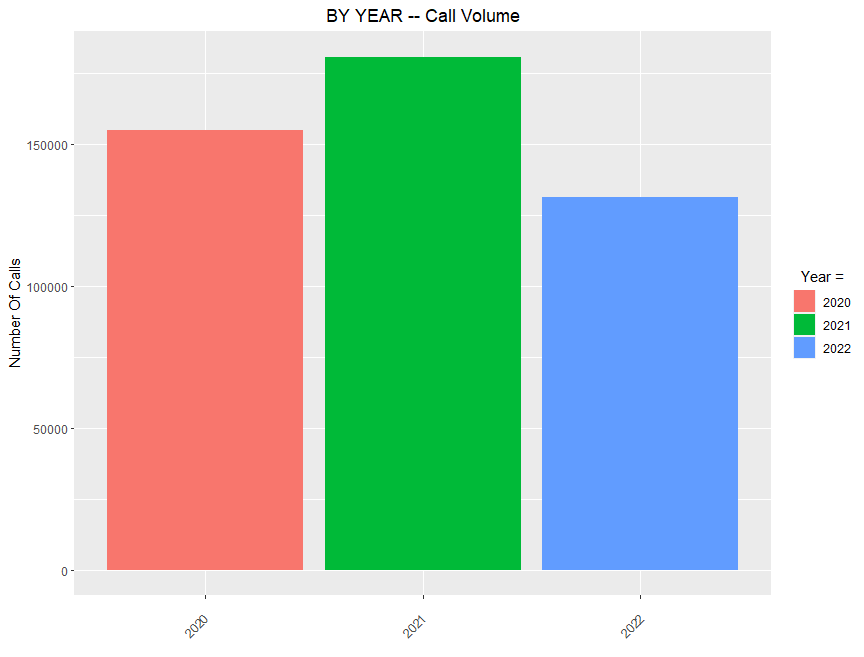
\includegraphics[width=200pt,height=200pt]{By Year.png}
    \caption{This is my first figure.}
    \label{fig:Year}
  \end{figure}

\section*{Results}
\citep{avramidis2005modeling}
\citep{evensen1999effective}
\citep{ibrahim2016modeling}

\section*{Results}

\section*{Discussion}


\bibliographystyle{chicago}
\bibliography{Citations.bib}
\end{document}